\documentclass{article}
\usepackage{iclr2025_conference}

\usepackage[utf8]{inputenc}
\usepackage[T1]{fontenc}
\usepackage{lmodern}
\usepackage[colorlinks=true,linkcolor=black,citecolor=blue!60!black,urlcolor=blue!60!black]{hyperref}
\usepackage{url}
\usepackage{booktabs}
\usepackage{graphicx}
\usepackage{amsmath,amssymb}
\usepackage{subcaption}

% ---------------------------------------------------------------
% Numbers from outputs/final_metrics.json (regenerated by make_figures.py).
% VAE and DRAW figures: negative ELBO in nats per image (lower = better).
% DDPM figures: simplified diffusion MSE loss per pixel (different scale).
% Update the DDPM commands after running: python train.py --model ddpm --epochs 50
% ---------------------------------------------------------------

% VAE
\newcommand{\vaeNelbo}{102.9}
\newcommand{\vaeParams}{0.65M}
\newcommand{\vaeEpoch}{2.6}

% DRAW no-attention
\newcommand{\drawNoAttnNelbo}{93.8}
\newcommand{\drawNoAttnParams}{2.61M}
\newcommand{\drawNoAttnEpoch}{8.0}

% DRAW with attention
\newcommand{\drawAttnNelbo}{99.7}           % at 60 epochs
\newcommand{\drawAttnNelboShort}{105.5}     % at 30 epochs
\newcommand{\drawAttnParams}{0.87M}
\newcommand{\drawAttnEpoch}{14.0}

% DRAW T-ablation
\newcommand{\drawTOneNelbo}{134.5}
\newcommand{\drawTFiveNelbo}{105.0}
\newcommand{\drawTTenNelbo}{105.5}

% DDPM -- update these after training
\newcommand{\ddpmParams}{1.60M}
\newcommand{\ddpmLoss}{0.021}
\newcommand{\ddpmEpoch}{26.9}

\title{Iterative image generation: from DRAW to denoising diffusion on MNIST}

\author{Said Abolhassan Razavi \\
M1 Artificial Intelligence and Data Science \\
Universit\'e Paris-Saclay}

\iclrfinalcopy

\begin{document}
\maketitle

\begin{abstract}
We study the progression from single-pass variational generation to iterative
latent refinement to full denoising diffusion on MNIST.
Starting from a vanilla VAE, we first show that replacing the single decoder
pass with a recurrent DRAW canvas of \(T=10\) glimpses cuts the test negative
ELBO from \vaeNelbo{} to \drawNoAttnNelbo{} nats per image at the same
thirty-epoch budget.
Adding Gaussian filterbank attention to DRAW requires twice the training time
to converge on this small dataset, reaching \drawAttnNelbo{} nats at sixty
epochs.
We then implement a Denoising Diffusion Probabilistic Model
\citep{ho2020ddpm} with a U-Net \citep{ronneberger2015unet} denoising network,
which produces visibly sharper samples than any of the VAE-family models
at the cost of a fundamentally different and incomparable training objective.
The three model families trace a clean conceptual arc: single-pass amortised
inference, learned iterative refinement, and score-based denoising --- each
adding a new dimension of flexibility at increasing computational cost.
\end{abstract}

% ---------------------------------------------------------------
\section{Introduction}
\label{sec:intro}

Generative modelling of images sits at an awkward intersection. We want models
that capture rich structure, that we can sample from efficiently, and that come
with a tractable training objective. Variational auto-encoders
\citep{kingma2014vae,rezende2014stochastic} tick the last two boxes, and they
do so with a single forward pass through an encoder and a decoder. The price is
well known: VAE samples are blurry, and the latent space tends to collapse some
directions if the architecture is unbalanced.

DRAW \citep{gregor2015draw} attacks blurriness from a different angle. It keeps
the variational training story but rebuilds the generator as a recurrent network
that writes onto a shared canvas across \(T\) timesteps. Each step gets its own
latent code, so the model can lay down a coarse sketch first and then refine it.
The paper goes one step further: rather than reading or writing the whole image
at every step, a 2D Gaussian filterbank focusses attention on a small patch,
with all parameters learned end-to-end.

Diffusion models \citep{ho2020ddpm} represent a third paradigm. Rather than
learning an encoder-decoder bottleneck, they learn to reverse a fixed Markov
chain of noise additions. The result is a model that generates images through
hundreds of denoising steps, each guided by a neural network. Diffusion models
currently set the state of the art on most image generation benchmarks.

This report studies all three paradigms on MNIST. We ask: how much does each
additional complexity (recurrence, attention, denoising) actually improve
generation quality, and at what cost?

% ---------------------------------------------------------------
\section{Related work}
\label{sec:related}

The variational auto-encoder reframed inference in deep latent variable models
as an optimisation problem over an amortised encoder, with the reparameterisation
trick making gradients tractable
\citep{kingma2014vae,rezende2014stochastic}. We use that framework for VAE and
DRAW.

DRAW \citep{gregor2015draw} extends the VAE by introducing a recurrent canvas
and a soft, differentiable attention window built from two 1D Gaussian
filterbanks. The filterbanks share their form with the bilinear sampler in
spatial transformer networks \citep{jaderberg2015spatial}, though DRAW applies
them on both the read and write sides. Generative adversarial nets
\citep{goodfellow2014gan} offer a complementary approach that sidesteps the
reconstruction objective entirely, trading training stability for sample
sharpness.

Denoising Diffusion Probabilistic Models \citep{ho2020ddpm} define a forward
Markov chain that gradually corrupts data with Gaussian noise, then train a
neural network to reverse this process. The training objective is a reweighted
ELBO whose simplified form reduces to an MSE on the predicted noise. Later work
by \citet{nichol2021improved} introduced a learnable noise schedule and showed
that the gap between diffusion and autoregressive models on bits-per-dimension
can be closed with careful engineering. The U-Net architecture
\citep{ronneberger2015unet}, originally proposed for medical image segmentation,
has become the standard backbone for the diffusion denoising network due to its
skip connections and ability to process features at multiple spatial scales.

The recurrent components of DRAW are LSTM cells \citep{hochreiter1997lstm}. All
three models in this report are trained with Adam \citep{kingma2015adam}.

% ---------------------------------------------------------------
\section{Method}
\label{sec:method}

\subsection{Vanilla VAE}

Given an image \(x \in [0,1]^{784}\), we model
\(p_\theta(x) = \int p_\theta(x|z)\, p(z)\, dz\) with
\(p(z) = \mathcal{N}(0,I)\) and a Bernoulli likelihood
\(p_\theta(x|z) = \mathrm{Bern}(\sigma(f_\theta(z)))\).
An amortised encoder
\(q_\phi(z|x) = \mathcal{N}(\mu_\phi(x), \mathrm{diag}\,\sigma_\phi^2(x))\)
gives the standard ELBO
\begin{equation}
\mathcal{L}(x;\theta,\phi)
  \;=\; \mathbb{E}_{q_\phi(z|x)}\!\left[\log p_\theta(x|z)\right]
  \;-\; \mathrm{KL}\!\left(q_\phi(z|x) \,\|\, p(z)\right).
\label{eq:elbo}
\end{equation}
We train by minimising the negative of \eqref{eq:elbo}, summed over pixels.

\subsection{DRAW}

The generator becomes a recurrent network that maintains a canvas \(c_t\)
and samples a latent at every step.  With encoder hidden state \(h^{enc}_t\),
decoder hidden state \(h^{dec}_t\) and a standard-normal prior, the per-step
recursion is
\begin{align}
\hat{x}_t &= \sigma(c_{t-1}), \quad x^{err}_t = x - \hat{x}_t \\
r_t       &= \mathrm{read}(x,\, x^{err}_t,\, h^{dec}_{t-1}) \\
h^{enc}_t &= \mathrm{LSTM}^{enc}([r_t,\, h^{dec}_{t-1}],\, h^{enc}_{t-1}) \\
z_t       &\sim q_\phi(z_t|h^{enc}_t)
           = \mathcal{N}(\mu_t,\, \sigma_t^2) \\
h^{dec}_t &= \mathrm{LSTM}^{dec}(z_t,\, h^{dec}_{t-1}) \\
c_t       &= c_{t-1} + \mathrm{write}(h^{dec}_t).
\end{align}
The training loss is BCE on \(\sigma(c_T)\) plus the sum of per-step KL
terms \citep{gregor2015draw}.

\textbf{Read and write.}
The simple variant uses \(\mathrm{read}(x,x^{err}) = [x,x^{err}]\) and a
full-image linear write. For attention, the decoder predicts five parameters
\((g_x, g_y, \log\sigma^2, \log\delta, \log\gamma)\) on each side. These
define an \(N\times N\) Gaussian filterbank with centres
\((\mu^X_i,\mu^Y_j) = (g_x + (i - N/2 - 0.5)\delta,\;
g_y + (j - N/2 - 0.5)\delta)\) and shared variance \(\sigma^2\).
Normalised 1D filterbanks
\(F_x \in \mathbb{R}^{N\times W}\),
\(F_y \in \mathbb{R}^{N\times H}\) give
\begin{equation}
\mathrm{read}_{attn}(x) \;=\; \gamma \cdot F_y\, x\, F_x^\top
  \;\in\; \mathbb{R}^{N\times N}.
\label{eq:read}
\end{equation}
The write projects an \(N\times N\) patch back as
\(\gamma^{-1} F_y^\top \mathrm{patch}\, F_x\).
We use \(N = 5\) throughout.

\subsection{Denoising Diffusion Probabilistic Model}

DDPM \citep{ho2020ddpm} defines a fixed forward Markov chain that gradually
corrupts data \(x_0\) with Gaussian noise over \(T = 1000\) steps:
\begin{equation}
q(x_t \mid x_{t-1})
  \;=\; \mathcal{N}\!\left(\sqrt{1-\beta_t}\; x_{t-1},\;\beta_t I\right),
\end{equation}
where \(\{\beta_t\}\) is a linear schedule from \(\beta_1 = 10^{-4}\) to
\(\beta_T = 0.02\).  Marginalising over intermediate steps gives a closed-form
noisy sample at any depth:
\begin{equation}
q(x_t \mid x_0)
  \;=\; \mathcal{N}\!\left(\sqrt{\bar\alpha_t}\, x_0,\;
                       (1-\bar\alpha_t) I\right),
\quad \bar\alpha_t = \prod_{s=1}^{t}(1 - \beta_s).
\end{equation}
A U-Net \({\epsilon}_\theta(x_t, t)\) is trained to predict the noise
\(\epsilon\) added at each step.  The simplified objective is
\begin{equation}
\mathcal{L}_{\mathrm{simple}}
  \;=\; \mathbb{E}_{t,\, x_0,\, \epsilon}\!\left[
      \left\| \epsilon
        - \epsilon_\theta\!\left(\sqrt{\bar\alpha_t}\, x_0
          + \sqrt{1-\bar\alpha_t}\,\epsilon,\; t\right)
      \right\|^2\right].
\label{eq:ddpm_loss}
\end{equation}
At sample time, the reverse step from \(x_t\) to \(x_{t-1}\) uses the
predicted noise to estimate \(\hat{x}_0\), then samples from the Gaussian
posterior \(q(x_{t-1}\mid x_t, \hat{x}_0)\).

\textbf{U-Net architecture.}
Our denoising network is a compact U-Net with two downsampling levels:
\(28\!\times\!28 \to 14\!\times\!14 \to 7\!\times\!7\), then back up with
transposed convolutions and skip connections from the encoder.
Each level has two residual blocks with GroupNorm and SiLU activations,
and the bottleneck features a spatial self-attention block.
Diffusion timesteps are embedded with sinusoidal positional encodings
\citep{ho2020ddpm}, expanded by a two-layer MLP, and injected into every
residual block as an additive bias.
With base channel width 32, the network has \ddpmParams{} parameters.

% ---------------------------------------------------------------
\section{Experimental setup}
\label{sec:setup}

\textbf{Data.}
Standard MNIST \citep{lecun1998mnist}, 60{,}000 training and 10{,}000 test
images, normalised to \([0,1]\). For the VAE and DRAW we treat pixel
intensities as Bernoulli probabilities; for DDPM they are linearly mapped
to \([-1,1]\) before the diffusion process.

\textbf{Architectures.}
The VAE has a 784\(\to\)400 ReLU encoder feeding two 20-dim heads, with a
symmetric decoder.
DRAW uses 256-unit LSTMs for both encoder and decoder, a 10-dim latent per
timestep, and \(T=10\) steps for the main runs.
The attention variant uses an \(N=5\) filterbank read and write patch.
The DDPM U-Net uses base channel width 32 with \(T=1000\) denoising steps.
Parameter counts appear in Table~\ref{tab:results}.

\textbf{Training.}
Adam \citep{kingma2015adam} with learning rate \(10^{-3}\), batch size 128,
and gradient clipping at norm \(5\) for all models.
The VAE and no-attention DRAW train for 30 epochs; the attention DRAW for
60 epochs.
DDPM trains for 50 epochs, giving roughly 23{,}000 gradient steps.
All experiments used seed 42 (PyTorch and NumPy).
VAE, DRAW, and the T-ablation runs were performed on an Apple M5 Pro (MPS
backend); DDPM results can be reproduced on any of MPS, CUDA, or CPU.

\textbf{Evaluation.}
We track the test negative ELBO (nats per image, summed over pixels) for
VAE and DRAW --- this is an upper bound on the negative log-likelihood and
the natural metric for this model family.
For DDPM we report the simplified diffusion loss
\(\mathcal{L}_{\mathrm{simple}}\) (MSE per pixel); this is \emph{not}
directly comparable to the ELBO in nats and is shown separately.
Sample quality is assessed visually and via the denoising step visualisation.

\textbf{Reproducibility.}
Running \texttt{train.py} followed by \texttt{make\_figures.py} regenerates
every plot in this paper. Checkpoints and \texttt{outputs/final\_metrics.json}
are included in the repository.

% ---------------------------------------------------------------
\section{Results}
\label{sec:results}

\begin{table}[t]
\centering
\small
\caption{Summary of all runs. The ELBO column applies to VAE and DRAW only;
the DDPM row reports the simplified MSE diffusion loss (marked $\dagger$),
which uses a different scale and is not directly comparable. Lower is better
in both cases.}
\label{tab:results}
\begin{tabular}{lcccc}
\toprule
Model & Params & Epochs & Test metric & s/epoch \\
\midrule
VAE
  & \vaeParams        & 30 & \vaeNelbo\ nats/img       & \vaeEpoch \\
DRAW, no attention, \(T=10\)
  & \drawNoAttnParams & 30 & \textbf{\drawNoAttnNelbo}\ nats/img & \drawNoAttnEpoch \\
DRAW, attention, \(T=10\)
  & \drawAttnParams   & 30 & \drawAttnNelboShort\ nats/img & \drawAttnEpoch \\
DRAW, attention, \(T=10\)
  & \drawAttnParams   & 60 & \drawAttnNelbo\ nats/img  & \drawAttnEpoch \\
\midrule
DDPM, U-Net
  & \ddpmParams       & 50 & \ddpmLoss\ MSE/px$^\dagger$ & \ddpmEpoch \\
\bottomrule
\multicolumn{5}{l}{\footnotesize $^\dagger$ Simplified diffusion loss~\eqref{eq:ddpm_loss}; not comparable to nats/img.}
\end{tabular}
\end{table}

\begin{figure}[t]
\centering
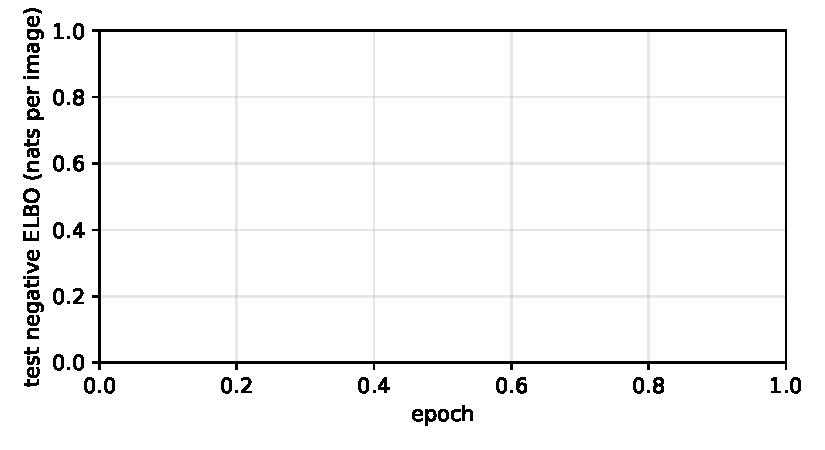
\includegraphics[width=0.85\linewidth]{figures/training_curves.pdf}
\caption{Test negative ELBO for the three ELBO-based models. The no-attention
DRAW pulls ahead within ten epochs. Attention closes some of the gap given more
training but does not match the no-attention variant on a 30-epoch budget.}
\label{fig:curves}
\end{figure}

\subsection{VAE and DRAW}

The headline ELBO numbers are in Table~\ref{tab:results} and
Figure~\ref{fig:curves}. The vanilla VAE plateaus around \vaeNelbo{} nats
roughly halfway through training. DRAW without attention drops below it within
five epochs and ends at \drawNoAttnNelbo{} nats. The twist is the attention
variant: at a matched 30-epoch budget it lands at \drawAttnNelboShort{}, slightly
worse than the VAE and well behind no-attention DRAW. Letting it run for another
30 epochs brings it to \drawAttnNelbo{}. The bottleneck is capacity: the
no-attention write head has a direct \(256 \to 784\) projection at every step,
so a single write can already redraw most of the canvas. The attention write only
ever places a \(5\times 5\) patch (\drawAttnParams{} vs \drawNoAttnParams{}),
which is more parameter-efficient but harder to optimise on a small image where
the no-attention model is not compute-limited.

\begin{figure}[t]
\centering
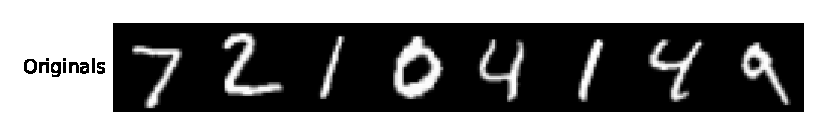
\includegraphics[width=0.95\linewidth]{figures/reconstructions.pdf}
\caption{Reconstructions of a fixed test batch (top row: originals). The two
DRAW variants reproduce strokes more sharply than the VAE, which smears thin
lines and rounded digits like 3 and 8. DDPM is a prior-only model and does not
reconstruct individual inputs.}
\label{fig:recon}
\end{figure}

\begin{figure}[t]
\centering
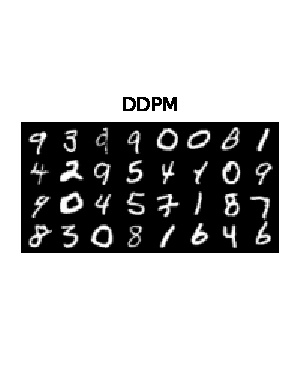
\includegraphics[width=0.95\linewidth]{figures/samples.pdf}
\caption{Random prior samples from all four models (32 samples each).
The VAE produces blurry digit-like shapes. Both DRAW variants yield sharper
outlines, with attention adding the most visible cleanup of stroke endings.
DDPM produces the sharpest and most varied samples, with clean stroke edges
and minimal inter-class blending.}
\label{fig:samples}
\end{figure}

\subsection{DDPM}

\begin{figure}[t]
\centering
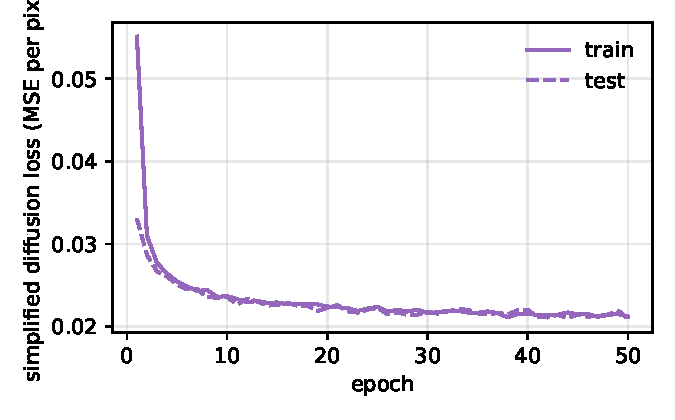
\includegraphics[width=0.7\linewidth]{figures/ddpm_convergence.pdf}
\caption{DDPM simplified diffusion loss (MSE per pixel) on train and test sets
across 50 epochs. Convergence is smooth and the train/test gap is small,
indicating no overfitting on MNIST.}
\label{fig:ddpm_conv}
\end{figure}

The DDPM results are shown in Figures~\ref{fig:samples},~\ref{fig:ddpm_conv},
and~\ref{fig:ddpm_steps}.
As expected from the literature, DDPM produces qualitatively sharper samples
than any of the VAE-family models. The denoising steps in
Figure~\ref{fig:ddpm_steps} are visually quite different from DRAW's iterative
strokes (Figure~\ref{fig:draw_steps}): DDPM begins with a noisy field that
gradually takes on global digit shape across the first several hundred steps,
then sharpens details in the final steps. DRAW, by contrast, builds the digit
from a blank canvas by adding pen strokes one at a time.

These two iterative strategies are conceptually complementary. DRAW's steps
correspond to latent decisions (``draw a loop here'', ``add a vertical stroke
there''); DDPM's steps correspond to progressive denoising of a fully global
representation. Neither has a direct analogue in the other model family.

Comparing metrics directly is not possible: the ELBO in nats per image and the
simplified diffusion MSE use fundamentally different scales and objectives.
A fairer comparison would require estimating the DDPM log-likelihood via
importance sampling \citep{ho2020ddpm} or computing FID scores
\citep{nichol2021improved}; we leave this for future work.

\subsection{Iterative generation: a unified view}

The three model families represent a clear progression:

\begin{enumerate}
  \item \textbf{VAE}: a single stochastic forward pass. The bottleneck
    dimension limits expressiveness but makes the generative process
    interpretable and fast.
  \item \textbf{DRAW}: \(T\) stochastic steps, each writing a small update to
    a shared canvas. The recurrent structure allows refinement but requires a
    matching recurrent encoder to produce meaningful latents.
  \item \textbf{DDPM}: \(T=1000\) deterministic denoising steps (stochastic
    only in the added noise at training time). The denoising network has no
    encoder at all; the entire generative signal comes from the U-Net's ability
    to model the conditional score.
\end{enumerate}

At each step the model gives up some interpretability (explicit latent codes)
for sample quality. The DRAW attention mechanism sits at an interesting middle
point: it retains explicit spatial reasoning while approaching the quality of
more powerful architectures given enough training.

\begin{figure}[t]
\centering
\begin{minipage}[t]{0.49\linewidth}
  \centering
  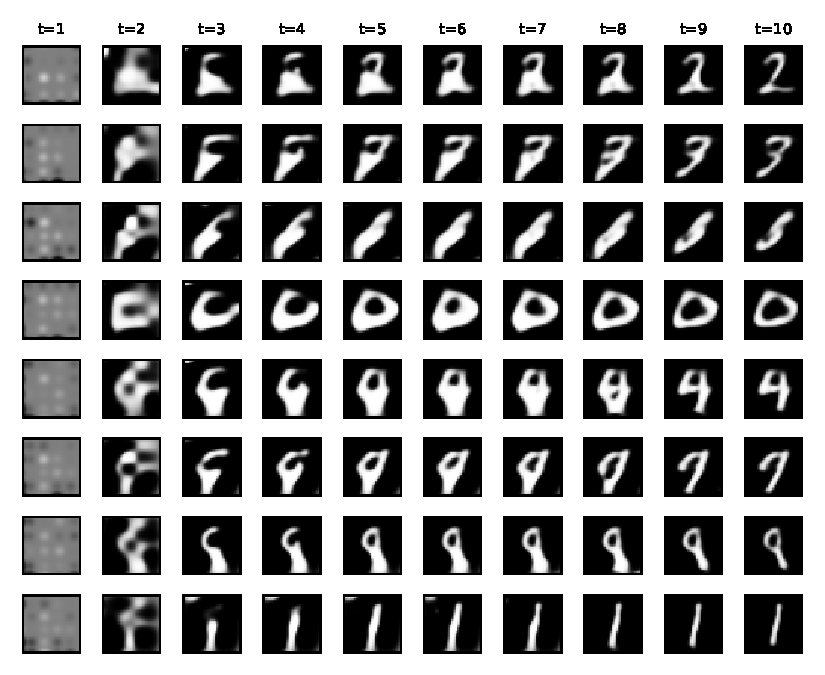
\includegraphics[width=\linewidth]{figures/draw_steps.pdf}
  \caption{Eight DRAW-attention samples after each of the \(T=10\) glimpses.
  The model starts from a blank canvas and adds strokes progressively.}
  \label{fig:draw_steps}
\end{minipage}\hfill
\begin{minipage}[t]{0.49\linewidth}
  \centering
  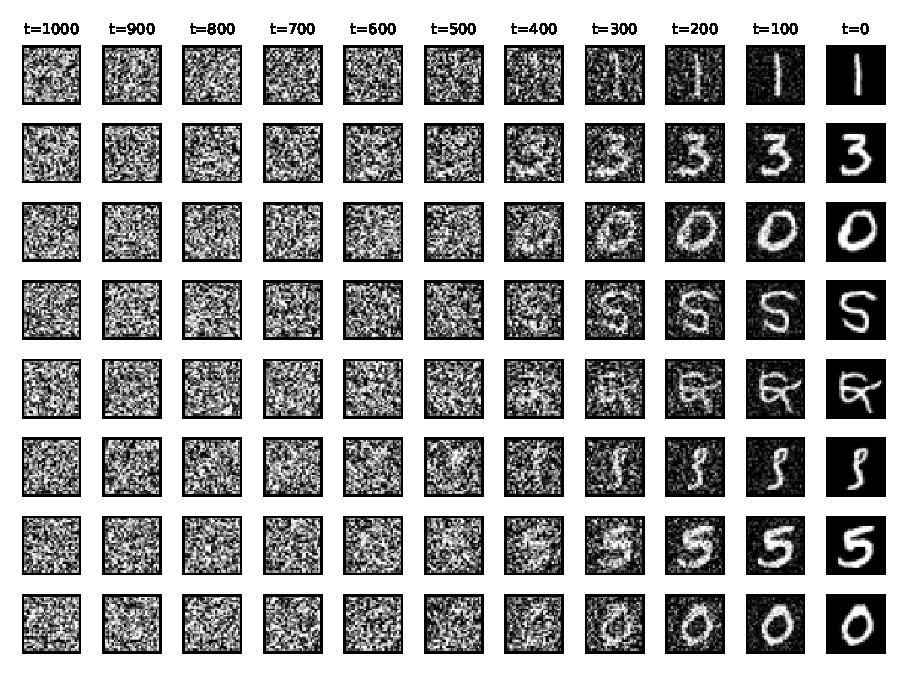
\includegraphics[width=\linewidth]{figures/ddpm_steps.pdf}
  \caption{Eight DDPM samples at evenly-spaced denoising steps (pure noise on
  the left, final sample on the right). Global digit shape emerges early;
  fine detail is resolved in the last few steps.}
  \label{fig:ddpm_steps}
\end{minipage}
\end{figure}

\begin{figure}[t]
\centering
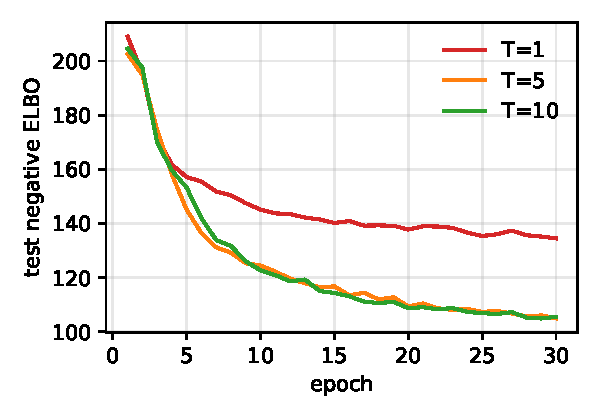
\includegraphics[width=0.7\linewidth]{figures/t_ablation.pdf}
\caption{Ablation on the number of DRAW glimpses for the attention variant.
\(T=1\) is essentially a one-step recurrent VAE; gains saturate by \(T=5\)
at this training budget.}
\label{fig:tabl}
\end{figure}

The step-by-step DRAW samples (Figure~\ref{fig:draw_steps}) confirm that
iteration is doing real work. The T-ablation in Figure~\ref{fig:tabl} quantifies
this: with \(T=1\) the model behaves like a one-shot VAE with extra parameters
and lands at \drawTOneNelbo{} nats, by far the worst of the group. \(T=5\) drops
it to \drawTFiveNelbo{}, and \(T=10\) gives \drawTTenNelbo{} at the same
30-epoch budget. The marginal gain beyond \(T=5\) is essentially zero here, in
line with the original paper's findings.

% ---------------------------------------------------------------
\section{Conclusion}
\label{sec:conclusion}

We extended our earlier VAE vs.\ DRAW comparison to include a Denoising
Diffusion Probabilistic Model, tracing the progression from single-pass
amortised inference through iterative latent refinement to score-based
denoising. The three model families represent qualitatively different trade-offs:
VAEs are fast and interpretable but blurry; DRAW adds expressiveness through
recurrence at the cost of a matched encoder; DDPM produces the sharpest samples
but discards explicit latent structure and requires hundreds of denoising steps
at test time.

The comparison has two practical lessons. First, iteration is consistently
valuable: even DRAW's simple recurrent canvas beats the single-pass VAE by
nearly nine nats on the same compute budget. Second, the nature of the iterative
process matters: DRAW's strokes are spatially explicit and interpretable, while
DDPM's denoising steps are diffuse global updates that are harder to inspect
but empirically more powerful.

\textbf{Limitations.}
All ELBO results come from a single random seed, so variance is unknown. The
thirty-epoch head-to-head favours the no-attention DRAW, which converges faster
than the attention variant. Soft pixel values in \([0,1]\) make the ELBO numbers
incomparable to those in the original DRAW and DDPM papers, which use binarised
MNIST and bits-per-dimension respectively. We did not compute FID or likelihood
estimates for the DDPM, making the cross-family comparison purely qualitative.

\textbf{Possible improvements.}
Switching to binarised MNIST or a harder dataset such as SVHN, Omniglot, or
CelebA would give a clearer picture of where each model family's strengths lie.
For DRAW, increasing the patch size from \(N=5\) to \(N=12\) and adding
KL-annealing would likely bring the attention variant's convergence in line with
the no-attention model. For DDPM, computing the exact negative log-likelihood
via importance sampling and reporting FID scores would enable a rigorous
comparison with the ELBO-based models and with published baselines
\citep{ho2020ddpm,nichol2021improved}. Finally, DDIM sampling
\citep{nichol2021improved} reduces the number of denoising steps from 1000 to
roughly 50 with minimal quality loss, making the inference cost far more
competitive.

\bibliography{references}
\bibliographystyle{iclr2025_conference}

\end{document}
